\documentclass[12pt]{article}

\title{Constraining the Supersonic Relative Velocity Effect on the Baryon Acoustic Oscillation Peak}
\author{Jenna Freudenburg \\
                Adviser: Nikhil Padmanabhan\\
                Yale University
}
\date{\today}

\usepackage{amsmath}
\usepackage{graphicx}
\usepackage{float}

\begin{document}
\maketitle

\begin{abstract} 
The goal of this project is to refine existing models for calculating the peak in the galaxy correlation function caused by baryon acoustic oscillations. We find that according to our model, depending on the value of the second-order bias parameter $b_{2}$, the position of the baryon acoustic oscillation peak may be shifted on the order of 0.1\% from its currently accepted value. This is a lower peak shift magnitude than the 1\% scale obtained by Yoo et al. in a recent study, and further study is needed to determine the cause of this discrepancy.
\end{abstract}

\tableofcontents

\section{Background}
\subsection{The primordial universe and the BAO}

During the era of inflation, the inflaton field experienced quantum density fluctuations. Due to the exponential expansion that occured during inflation, the scale of these fluctuations was rapidly magnified, creating small macroscopic density fluctuations that persisted after the end of inflation. This resulted in areas of overdensity, which over time accreted matter through gravitation, resulting in the large-scale structure we see in the universe today.

Post-inflation, the early universe consisted of primordial plasma, composed initially of quarks and gluons and later of free protons and electrons that interacted with photons via Thompson scattering. During this era, the photon-baryon interactions resulted in pressure variations that caused compressions and rarefactions throughout the cosmic fluid. These acoustic oscillations, centered at each overdensity and balanced by their gravitation, continued until recombination, which occured at approximately $3\times10^{5}$ years after the Big Bang \cite{Eisenstein}. At this point, the universe had cooled to approximately 3000 K. The matter and photons ceased to interact, and the photons free-streamed throughout the universe, which we see today as the cosmic microwave background. As a result, the pressure-driven acoustic oscillations ceased, leaving propagating overdensities of baryons essentially fixed at their last scatter positions -- a length scale referred to as the "sound horizon". Over time, these overdensities accreted gravitationally to form galaxies, and thus by measuring galactic positions today, we can detect this sound horizon and use it as a characteristic cosmic length scale. 

This evolution can be best understood by first analyzing the behavior of a single overdensity. Consider a single density perturbation propagating outward when recombination occurs. The mass profile of the baryons then looks like a peak at approximately 150 Mpc. Over time, this locus of matter attracts more matter to itself, while the dark matter (which only interacts gravitationally and is therefore not subject to pressure variations and acoustic oscillation) remains at the original overdense center and also accretes gravitationally, resulting in a mass profile evolution like that shown in Figure \ref{peakEvol} from Eisenstein et al \cite{Eisensteinetal}. Over many inital perturbations, then, we expect to see a preferred separation distance among galaxies. Studies have calculated the correlation function over large galaxy samples from the Sloan Digital Sky Survey (SDSS) and found a peak attributable to the BAO at a horizon of 150 Mpc \cite{Eisensteinetal}. This corresponds to a preferred angular separation, which was recently measured by Planck to be $0.596724\,^{\circ}\pm 0.00038\,^{\circ}$ \cite{Planck}. This characteristic scale can be used as a standard ruler for measuring cosmic acceleration independent of supernovae standard candles (which have been used in the past for cosmic measurement), and as such the BAO provides an important tool for the study of dark energy.

\begin{figure}[H]
	\centering
	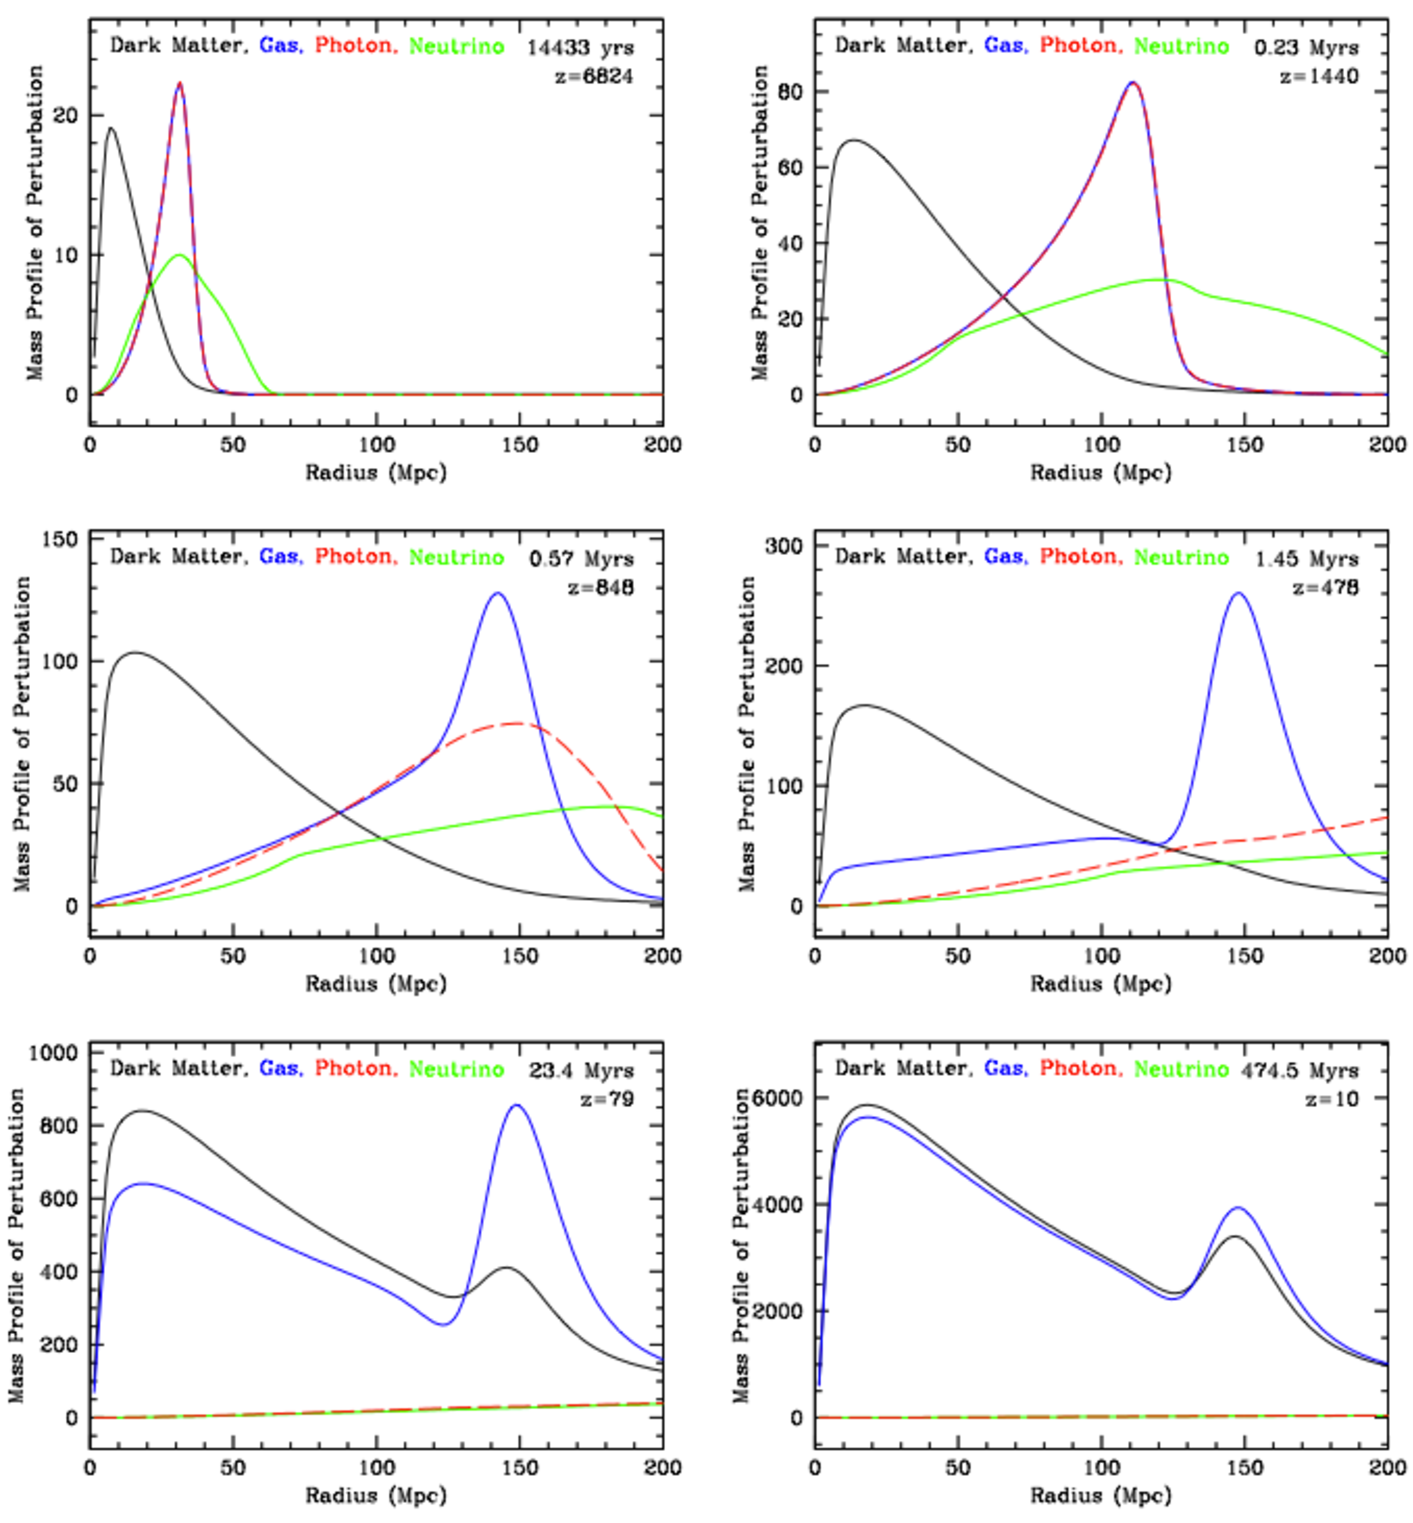
\includegraphics[width=13cm]{peakEvol}
	\caption{From Eisenstein et al \cite{Eisensteinetal}, the evolution of the BAO peak position over time. The mass function of different species existing in the early universe is shown in arbitrary units scaled for comparison. Reading across: a) Shortly after initial time of perturbation, the photons and baryons travel outward while the dark matter remains near the center; b) this outgoing pulse causes a wake in the dark matter; c) recombination, as the photons cease scattering and stream away from the baryonic matter; d) recombination complete, the baryonic and dark matter peak stand sharply at the center and at a fixed radius; e) each these two overdensities gravitationally attract one another, causing their mass profiles to become more similar; and f) the mass profiles approach what we measure today.}
	\label{peakEvol}
\end{figure}

\subsection{The supersonic relative velocity effect}
The most basic model for analyzing the BAO assumes Gaussian statistics and linear perturbations. This model is well-understood; however, higher-order corrections are necessary to constrain the BAO measurement to a precision that is useful for cosmological observations. Tseliakhovich and Hirata first proposed that a significant 2nd-order contribution to the BAO feature arises from the supersonic velocity of the dark matter fluid relative to the baryonic fluid after recombination \cite{TsHirata}. In theory, this relative velocity effectively raises the Jeans mass (the critical mass at which a cloud of matter collapses under gravity) and thus delays the formation of baryonic structure. Such a delay in structure formation would alter the power spectrum measured over galaxy distributions that exhibit this effect, resulting in a shift in the BAO peak. 

\subsection{Statistics}
Naturally, since we are looking for this effect over a large distribution of galaxies, we must analyze the distribution statistically in order to perceive the existence of a characteristic length scale. To linear order, this is most effectively achieved using the galaxy correlation function, which Peebles defines as follows: ``Given a random galaxy in a location, the correlation function describes the probability that another galaxy will be found within a given distance''\cite{Peebles}. More technically, the correlation function is given by $\left<\delta_{g}({\bf x_{a}})\right>\left<\delta_{g}({\bf x_{b}})\right>$, where $\delta_{g}$ denotes the galactic density constrast given by
\begin{equation}
\delta({\bf x})=\frac{\rho({\bf x})-\bar{\rho}}{\bar{\rho}}
\end{equation}
Under a Fourier transform, the galaxy correlation function gives the galaxy power spectrum, a common cosmological tool. Similarly, the most straightforward way to see the existence of non-Gaussian effects in a distribution is to examine its higher order cumulants -- specifically the three-point correlation function given by $\left<\delta_{g}\right>\left<\delta_{g}\right>\left<\delta_{g}\right>$. We note that this will give zero for cases where the density contrast distribution is Gaussian, and thus the existence of a bispectrum signal indicates a nonlinear effects in the galaxy distribution. As in the two-point case, it is often useful to examine the Fourier-space correlate of this statistic, known as the bispectrum \cite{Bernardeau}.

In a recent study, Yoo et al. further explore the non-Gaussianity introduced by the supersonic relative velocity effect using standard perturbation theory methods \cite{Yooetal}. Most importantly, they compute explicit equations for the galaxy power spectrum and bispectrum in order to compare these statistics to results from existing non-linear models of the BAO feature.

\section{Calculations and results}
\subsection{Power spectrum}
The CAMB software (Code for Anisotropies in the Microwave Background) was used to generate a linear matter power spectrum from a fiducial cosmology given in Yoo et al \cite{Yooetal}. Similary, CLASS (Cosmic Linear Anisotropy Solving System) was used to generate $T_{ru}$, the transfer function for relative velocity. These are both more up-to-date than CMBFAST, the system used by Yoo et al, so by using data from these alternate software packages we hope to be able to confirm some of their results.

Following Yoo et al., we assume a second-order term in the galaxy density fluctuation as follows:
\begin{equation}
\delta_{g}(\textbf{x}) = b_{1}\delta_{m}(\textbf{x})+\frac{b_{2}}{2} [\delta_{m}^{2}(\textbf{x})-\sigma_{m}^{2}]+\frac{b_{3}}{3!}\delta_{m}^{3}(\textbf{x})+b_{r} [u_{r}^{2}(\textbf{x})-\sigma_{ru}^{2}]
\end{equation}
where $u_{r} =\textbf{v}_{r}/\sigma_{rv}$ and $\sigma_{rv}$ is the one-dimensional rms relative velocity fluctuation. Then using standard perturbation theory, the equation for the full power spectrum is calculated to be 

\begin{eqnarray}
P_{g}(k) = b_{1}^{2}P_{nl}({\bf k}) + \int\frac{d^{3}\bf q}{(2\pi)^{3}}P_{m}(q)P_{m}(|{\bf k-q}|)[\frac{1}{2}b_{2}^{2}+2b_{1}b_{2}F_{2}({\bf q, k- q}) \\
+4b_{1}b_{r}F_{2}({\bf q, k- q})G_{u}({\bf q, k- q})+2b_{2}b_{r}G_{u}({\bf q, k- q})+2b_{r}^{2}G_{u}({\bf q, k- q})^{2}]
\nonumber \end{eqnarray}
where
\begin{eqnarray}
&&\int\frac{d^{3}\bf q}{(2\pi)^{3}}P_{m}(q)P_{m}(|{\bf k - q}|) F_{2}({\bf q, k- q}) \\
&&= \frac{k^{3}}{(2\pi)^{2}}\int_{0}^{\infty}dr\: r^{2}\: P_{m}(kr)\int_{-1}^{1}d\mu\: P_{m}\;(k\sqrt{1+r^{2}-2r\mu})\:\frac{3r+7\mu-10r\mu^{2}}{14r(1+r^{2}-2r\mu)}
\nonumber \end{eqnarray}
and 
\begin{eqnarray}
&&\int \frac{d^{3}\bf q}{(2\pi)^{3}}P_{m}(q)P_{m}(|{\bf k - q}|) G_{u}({\bf q, k- q}) \\
&&= \frac{k^{3}}{(2\pi)^{2}}\int_{0}^{\infty}dr\: r^{2}\: P_{m}(kr)\int_{-1}^{1}d\mu\: P_{m}\;(k\sqrt{1+r^{2}-2r\mu}) \nonumber \\
&&\times\;\frac{T_{ru}(q)}{T_{m}(q)}\:\frac{T_{ru}(k\sqrt{1+r^{2}-2r\mu})}{T_{m}(k\sqrt{1+r^{2}-2r\mu}))}\frac{r-\mu}{\sqrt{1+r^{2}-2r\mu})} 
\nonumber \end{eqnarray}

where $P_{m}$ is the linear matter power spectrum and $F_{2}$ and $G_{u}$ are the density field and velocity divergence field kernels, as found in Bernardeau et al. \cite{Yooetal}\cite{Bernardeau}. The numerical integration software Cuba was used to  explicitly calculate the value of this equation from the CAMB-generated linear power spectrum. We make the coordinate transformation $r \to 1/r $, so we have
\begin{equation}
\int_{0}^{\infty} f(r) dr = \int_{0}^{1} f(r) dr + \int_{1}^{\infty} f(r) dr = \int_{0}^{1} f(r) dr +\int_{0}^{1} r^{-2} f(1/r) dr
\end{equation}
This allows us to integrate out to infinity with Cuba. The full power spectrum, broken down term by term, is shown in Figure \ref{PSbd}. We note that the contribution of higher order terms, while small, is distinctly present in the full power spectrum when compared to the linear power spectrum. However, as outlined above, we expect that this effect will show up more prominently in the bispectrum.  

\begin{figure}[h]
	\centering
	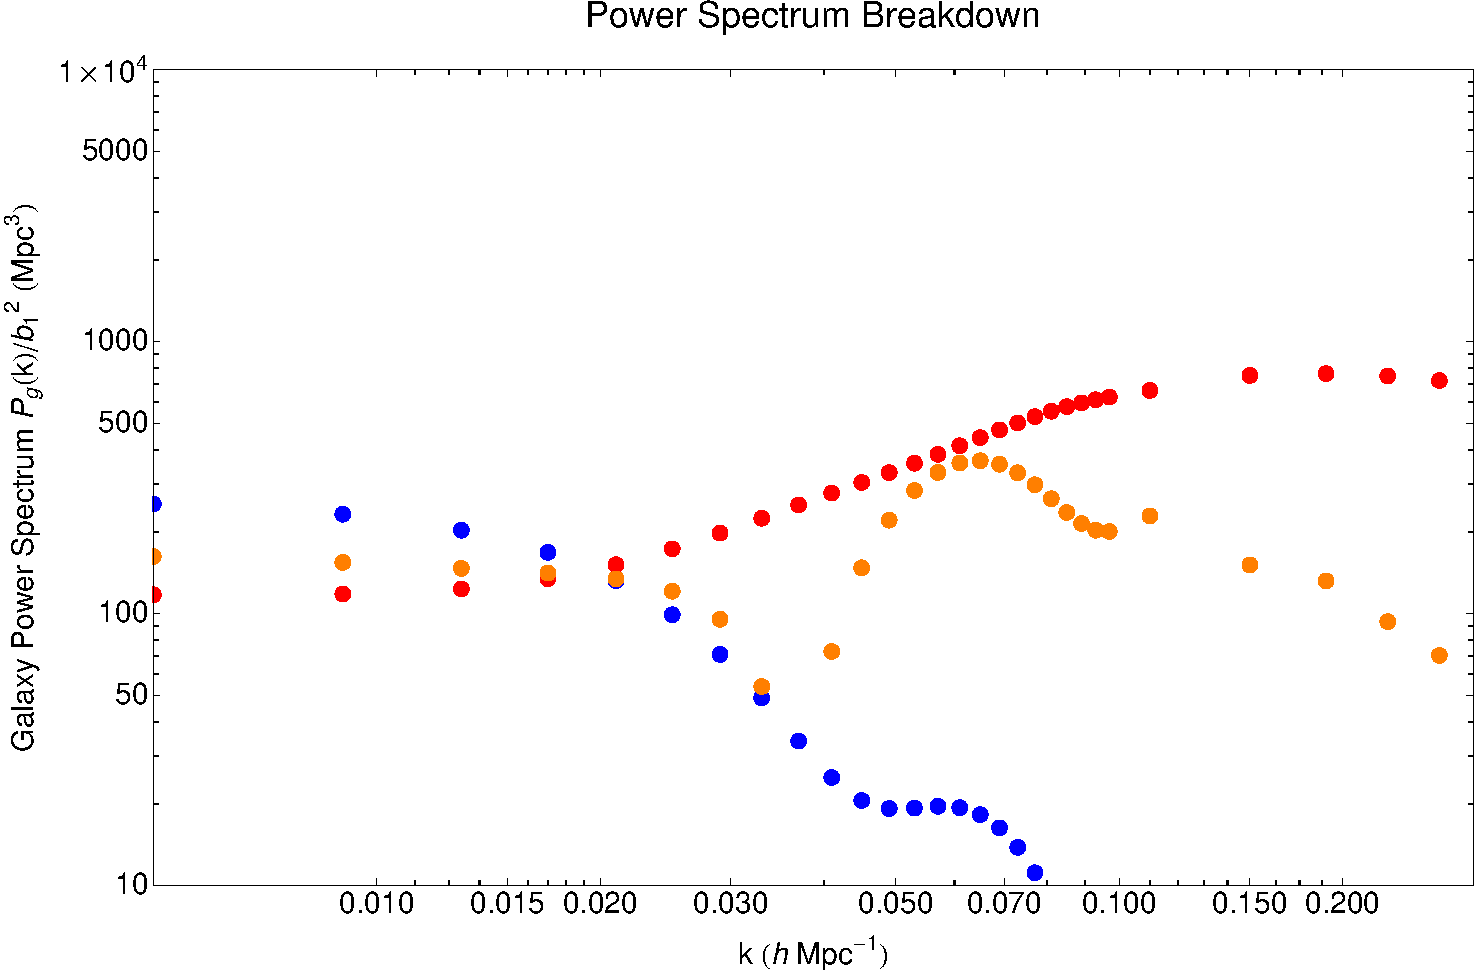
\includegraphics[width=16cm]{PSbd}
	\caption{The full galaxy power spectrum.}
	\label{PSbd}
\end{figure}

\subsection{BAO peak shift}
Once we have a full power spectrum complete with second-order terms, we may use it as input for an n-body simulation in order to impose a certain set of statistics. The code we use, from Manera et al \cite{Manera}, fits the power spectrum over a selection from 600 mock data sets that resemble the galaxy distribution in the real universe. From these fits (to the correlation functions of these data sets), the code can give higher order bias parameter $b_{2}$. Thus, by running the simulation many times for different values of $b_{r}$, we can generate mock data for the dependence of $b_{2}$ on $b_{r}$ in order to test Figure 5 in Yoo et al \cite{Yooetal}. In order to do this, we wrote a program to generate spectra based on Equation 3 for many different values of $b_{r}$. (Both bias parameters have been scaled to $b_{1}$, which we take to be 1.) The results are shown in Figure \ref{bplots}; compare with Yoo et al's prediction in Figure \ref{yds_bplots}. We readily observe a discrepancy for values of $b_{2}<0$. In Yoo et al, these relations exhibit a downward trend for values of $b_{r}>0.02$, a feature which does not appear in our analysis. Furthermore, the amplitude of the effect we detect is shallower; at $b_{r}=0.01$ and $b_{2}=0.2$, Yoo et al predict a 1\% upward shift in peak position, whereas we find a shift only on the scale of 0.1\%. One possible reason for these discrepancies could be a difference in fitting procedures, specifically in the ``no-wiggle'' smoothed power spectrum that is used as a baseline for the fits; another point of difference occurs in our use of numerical simulation rather than a direct fit. Further analysis is needed to determine the reason for these discrepancies. However, we also note that our trends do indicate a measurable shift in the peak position due to the supersonic relative velocity effect.

\begin{figure}[h]
	\centering
	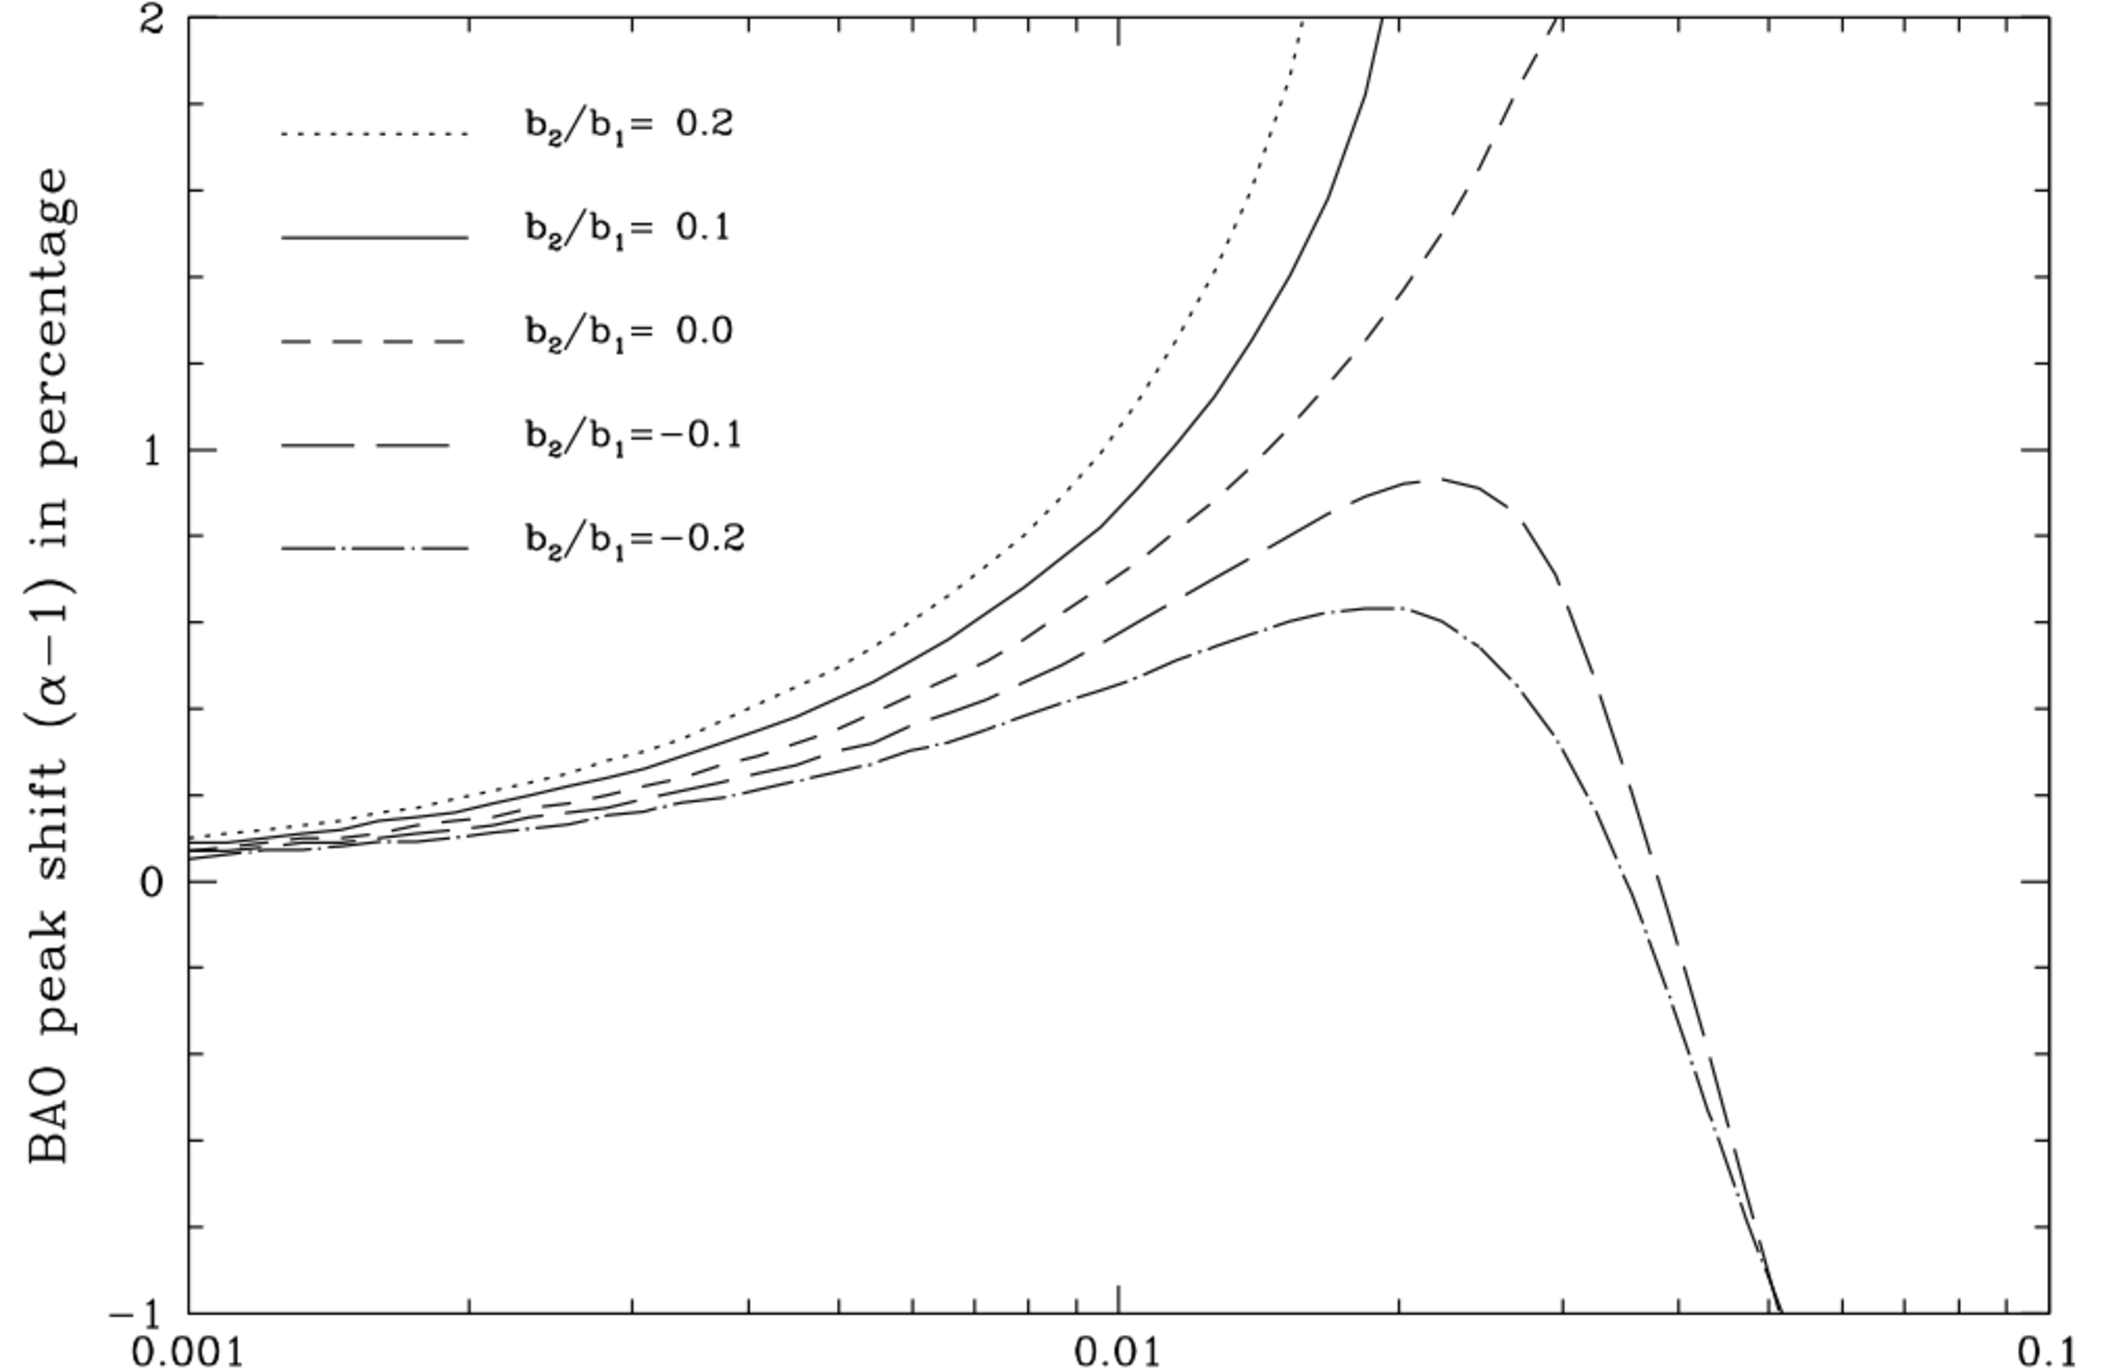
\includegraphics[width=14cm]{yds_bplots}
	\caption{Yoo et al's calculation of the BAO peak shift as a function of $b_{r}$ for different values of of $b_{2}$ \cite{Yooetal}.}
	\label{yds_bplots}
\end{figure}

\begin{figure}[h]
	\centering
	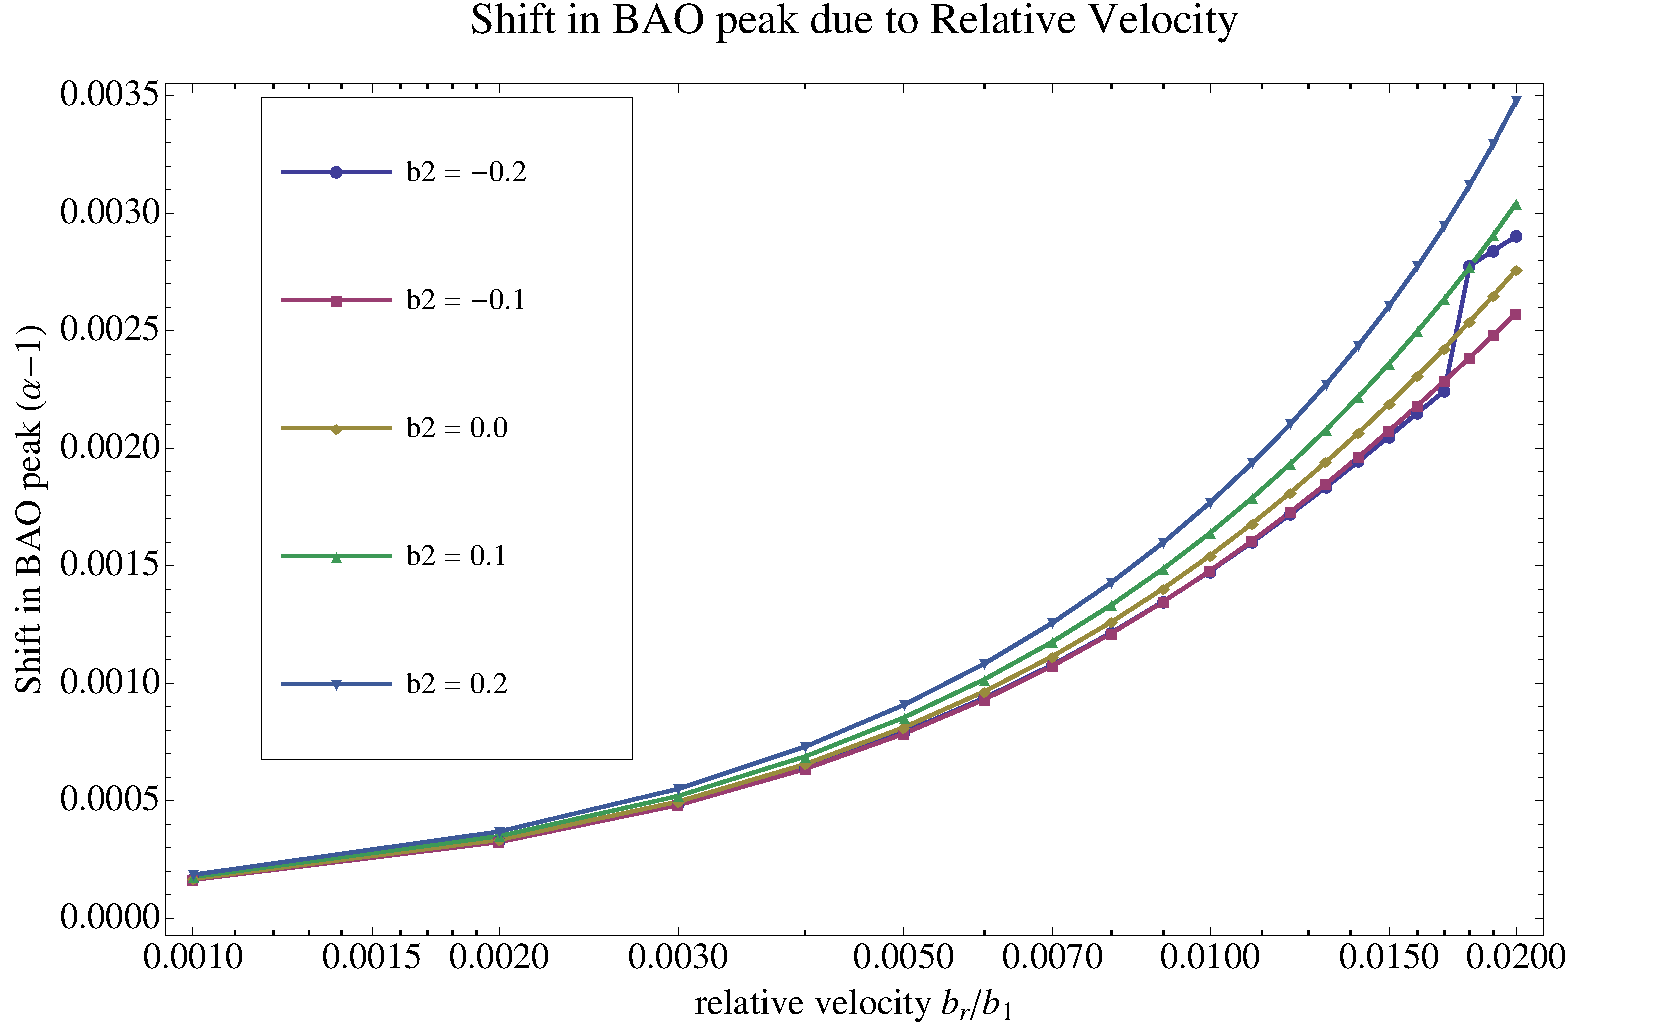
\includegraphics[width=14cm]{bplots}
	\caption{The shift in the BAO peak position for different values of the galaxy bias parameter $b_{2}$ as a function of $b_{r}$.}
	\label{bplots}
\end{figure}

\subsection{Bispectrum}

The bispectrum is given by the following equation, after Yoo et al:
\begin{eqnarray}
B_{g}({\bf k}_{a}, {\bf k}_{b}, {\bf k}_{c})&=&b_{1}^3  [2P_{m}(k_{a})P_{m}(k_{b})F_{2}({\bf k}_{a},{\bf k}_{b}) + cycl.] \\
&+& \frac{1}{2}b_{1}^{2}b_{2}[P_{m}(k_{a})P_{m}(k_{b}) + cycl.] + b_{1}^{2}b_{r}[2P_{m}(k_{a})P_{m}(k_{b})G_{u}({\bf k}_{a},{\bf k}_{b}) + cycl.] \nonumber \\
&+& 8b_{r}^{3}   \int{\frac{d^{3}{\bf q}}{(2\pi)^{3}}  P_{m}(|{\bf k}_{a}+{\bf q}) P_{m}(|{\bf k}_{b} - {\bf q})P_{m}(q) \nonumber \\
&\times&G_{u}({\bf k}_{a}+{\bf q},{\bf k}_{b}-{\bf q})G_{u}({\bf k}_{a} + {\bf q}, {\bf q})G_{u}({\bf q}, {\bf k}_{b}-{\bf q})
\nonumber \end{eqnarray}
Our calculations for the bispectrum were done assuming an equilateral triangle, such that $k_{a}=k_{b}=k_{c}=k$ and $\mu={\bf k}\cdot{\bf k}=-0.5$. As before, the linear power spectrum was obtained from CAMB. The result shown in Figure \ref{bspec} agrees quite well with Figure 3 in Yoo et al, which is to be expected given the relatively small differences in the power spectra we obtain relative to theirs. 

\subsection{Future work}

Once the discrepancies we have so far uncovered have been resolved, it would be useful to modify the simulation code to take in a bispectrum and analyze the three-point function for various triangular configurations of galaxies. The ultimate goal would be to obtain tight constraints on the second order bias parameters  and then run this study on galaxy distributions from real data. This would allow us to determine the impact of the relative velocity effect on the BAO feature in our own universe, and thus to account for it accurately when using the BAO as a cosmological tool. 

\begin{figure}[H]
	\centering
	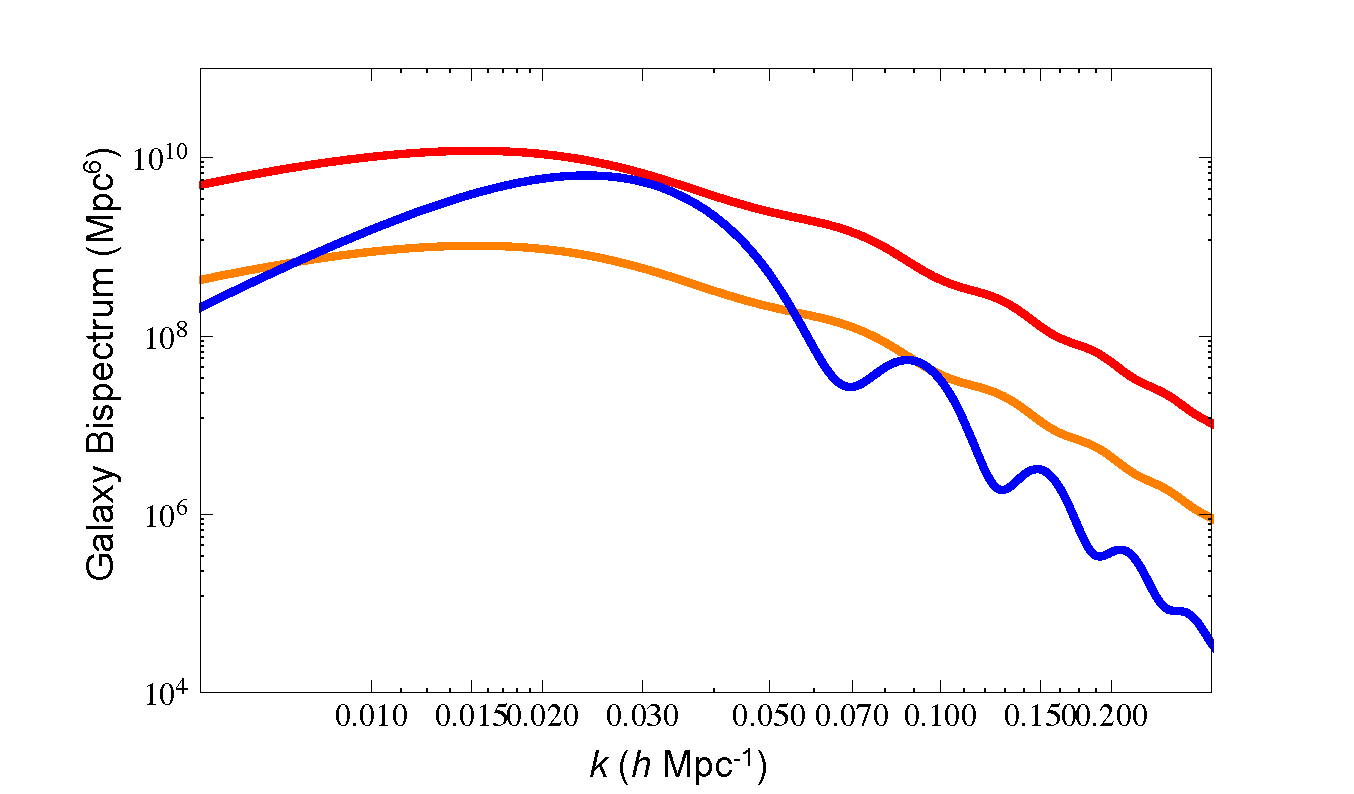
\includegraphics[width=16cm]{bspec}
	\caption{The full galaxy power spectrum (blue = auto-relative velocity term, orange = cross power terms, red = matter terms).}
	\label{bspec}
\end{figure}

\begin{thebibliography}{1}

\bibitem{TsHirata}
D. Tseliakhovich and C. Hirata, \emph{Relative velocity of dark matter and baryonic fluids and the formation of the first structures}, Phys. Rev. D \textbf{82}, 083520 (2010).

\bibitem{Eisensteinetal} 
D. Eisenstein et al., \emph{Detection of the baryon acoustic peak in the large-scale correlation function of SDSS luminous red galaxies}, Astrophys. J. \textbf{633}, 2 (2005).

\bibitem{Yooetal} 
J. Yoo, N. Dalal, and U. Seljak, \emph{Supersonic relative velocity effect on the baryonic acoustic oscillation measurements}, J. Cosmol. Astropart. Phys. \textbf{7}, 018 (2011). 

\bibitem{Szapudi}
I. Szapudi, \emph{Three-point statistics from a new perspective}, Astrophys. J. \textbf{605}, 2 (2004).

\bibitem{Planck}
Planck collaboration, \emph{Planck 2013 results. XVI. Cosmological parameters}, submitted, 	arXiv:1303.5076 (2013).

\bibitem{Eisenstein}
D. Eisenstein, "Proceedings of 'Probing the Dark Universe with Subaru and Gemini'". November 6-9, 2005 AGENDA Waikoloa, Hawaii. http://www.noao.edu/meetings/subaru, p.9.1

\bibitem{Bernardeau}
F. Bernardeau et al., \emph{Large-Scale Structure of the Universe and Cosmological Perturbation Theory}, arXiv:astro-ph/0112551v1 (2001).

\bibitem{Peebles}
P.J.E. Peebles, \emph{The large-scale structure of the universe}, Princeton Univ. Press (1980).

\bibitem{Manera}
M. Manera et al., \emph{The clustering of galaxies in the SDSS-III Baryon Oscillation Spectroscopic Survey: a large sample of mock galaxy catalogues}, Monthly Notices of the Royal Astronomical Society, \textbf{428}, 2 (2012).

\end{thebibliography}

\end{document}